\documentclass[12pt]{scrartcl}
\usepackage{graphicx}
\usepackage[default]{opensans}
\usepackage{sfmath} % sans font also for math
 \usepackage[binary-units = true]{siunitx}

% defining the paper layout that no text overlaps with the header
\usepackage[
  top=35mm,
  headheight=25mm,
  headsep=3mm,
  bottom=30mm,
  left=25mm,
  right=25mm
]{geometry}

\usepackage{latexsym}
\usepackage[centertags]{amsmath}
\usepackage{amssymb}

% custom header and footpage
\usepackage{scrpage2}
\pagestyle{scrheadings} % you have to set the custom layout
\ihead{M4.1: Simulation modules and interfaces } % left head
\ohead{
\includegraphics[height=25mm]{EUCALL.png}}
\ifoot{
\includegraphics[height=13.4mm]{EU.png}} % left foot
\cfoot{%
  \begin{minipage}{100mm}%
    \begin{scriptsize}%
      \normalfont{This project has received funding from the}
      \textit{European Union’s Horizon 2020 research and innovation programme}
      \normalfont{under grant agreement No 654220.}
    \end{scriptsize}%
  \end{minipage}%
} % center foot
\ofoot{} % right foot
\chead{}

\usepackage{booktabs}

% sophisticated linking of references in the pdf and setting some options
\usepackage{url}                                                  % for correct typesettings of URLs
\usepackage{hyperref}                                             % for sophisticated linking of urls, dois, pictures, tables, etc.
\hypersetup{
    unicode=true,                                                 % non-Latin characters in Acrobat’s bookmarks
    pdftoolbar=true,                                              % show Acrobat’s toolbar?
    pdfmenubar=true,                                              % show Acrobat’s menu?
    pdffitwindow=false,                                           % window fit to page when opened
    pdfstartview={FitH},                                          % fits the width of the page to the window
    pdftitle={M4.1: Simulation modules and interfaces},           % title
    pdfauthor={C. Fortmann-Grote},                                % author
    pdfsubject={EUCALL WP4 (SIMEX) Milestone 4.2},                % subject of the document
    pdfcreator={pdflatex},                                        % creator of the document
    pdfkeywords={EUCALL, SIMEX, simulations, PIC, XFEL, scattering},                                         % list of keywords
    pdfnewwindow=true,                                           % links in new PDF window
    colorlinks=true,                                             % false: boxed links; true: colored links
    linkcolor=blue,                                              % color of internal links (change box color with linkbordercolor)
    citecolor=blue,                                              % color of links to bibliography
    filecolor=blue,                                              % color of file links
    urlcolor=blue                                                % color of external links
}


% for fast reference
\newcommand{\fig}[1]{{figure\,\ref{#1}}}
\newcommand{\tab}[1]{{table\,\ref{#1}}}
\newcommand{\eq}[1]{{equation~(\ref{#1})}}


% Zeilenabstand
\renewcommand{\baselinestretch}{1.2}


%%%%%%%%%%%%%%%%%%%%%%%%%%%%%%%%%%%%%%%%%%%%%%%
%   BIBLIOGRAPHY SETTINGS                     %
%%%%%%%%%%%%%%%%%%%%%%%%%%%%%%%%%%%%%%%%%%%%%%%
\usepackage[bibstyle=nature,sorting=none,=maxnames=1000,eprint=false,
defernumbers=true, backend=biber]{biblatex}
\usepackage{hyperref}

\renewcommand*\finalnamedelim{, and\addspace}
\DeclareNameAlias{sortname}{last-first}
\renewcommand{\newunitpunct}{, }

\AtEveryBibitem{%
  \clearfield{day}%
  \clearfield{month}%
  \clearfield{endday}%
  \clearfield{endmonth}%
  \clearfield{issn}%
  \clearfield{issue}%
}
%convert titles to hyperlinks using doi
\ExecuteBibliographyOptions{doi=false} \newbibmacro{string+doi}[1]{%
  \iffieldundef{doi}{#1}{\href{http://dx.doi.org/\thefield{doi}}{#1}}}
  \DeclareFieldFormat*{title}{\usebibmacro{string+doi}{\mkbibemph{#1}}}

%\addbibresource{/home/grotec/Documents/LiteratureDB/bibtex/jabref.bib}
\addbibresource{/home/carsten/Documents/LiteratureDB/bibtex/jabref.bib}
%\addbibresource{references.bib}
%%%%%%%%%%%%%%%%%%%%%%%%%%%%%%%%%%%%%%%%%%%%%%%
% END BIBLIOGRAPHY SETTINGS                   %
%%%%%%%%%%%%%%%%%%%%%%%%%%%%%%%%%%%%%%%%%%%%%%%

\begin{document}
\makeatletter
\begin{titlepage}
\thispagestyle{scrheadings}
\begin{center}
$~$\\
\vspace{2cm}
\Huge{\textbf{WP 4 -- SIMEX\\[1cm]
Milestone M4.1: Delivery of individual simulation modules and common interfaces
for interoperability}}\\[5mm]
\vspace{2cm}
\large{
Carsten Fortmann-Grote, Alexander Andreev, Richard Briggs,\\ Michael Bussmann,
  Axel Huebl, Thomas Kluge,\\
 S. Pascarelli, Ashutosh Sharma, and Adrian P. Mancuso\\
 }
\vspace{1cm}
\@date
\end{center}
\vfill%

\includegraphics[width=\textwidth]{./PartnerLogos.pdf}
\normalfont
\end{titlepage}
\makeatother

%
\section{Introduction}
The computer program \texttt{simex\_platform} \cite{simex_github} is a modular
software environment for the simulation of experiments at advanced laser light
sources. It allows the user to assemble a virtual experiment through combination
of suitable programs for the light source (e.g. a synchrotron, an x-ray free
electron laser, or an optical laser), beam transport from the source to the
sample or target, interaction of the light with the sample or target,
propagation of the scattered light behind the sample or target, and detection in
a light detector. \texttt{simex\_platform} comes preloaded with a number of such
\textit{Calculators}, aimed at the simulation of various typical laser light
experiments. Furthermore, researchers can replace individual built-in
\textit{Calculators} by their own codes. In this way, they can embed their codes
into a more realistic simulation environment compared to running the code in
stand-alone fashion with more or less idealized param

\subsection{The EUCALL Software repository}
github, other codes.

\subsection{Software requirements}
\texttt{simex\_platform} is implemented in the python programming language. To
ensure support on as many hardware platforms and operating systems as possible,
we chose python 2.7. The software requirements for
\texttt{simex\_platform} as well as for the backengine calculators that ship
with it can be found on the github repository \cite{simex_github} and are listed
in the appendix.
%
\section{Modular structure of virtual photon experiments and simulation
  \textit{Calculators}}
\begin{figure}[ht]
  \begin{center}
    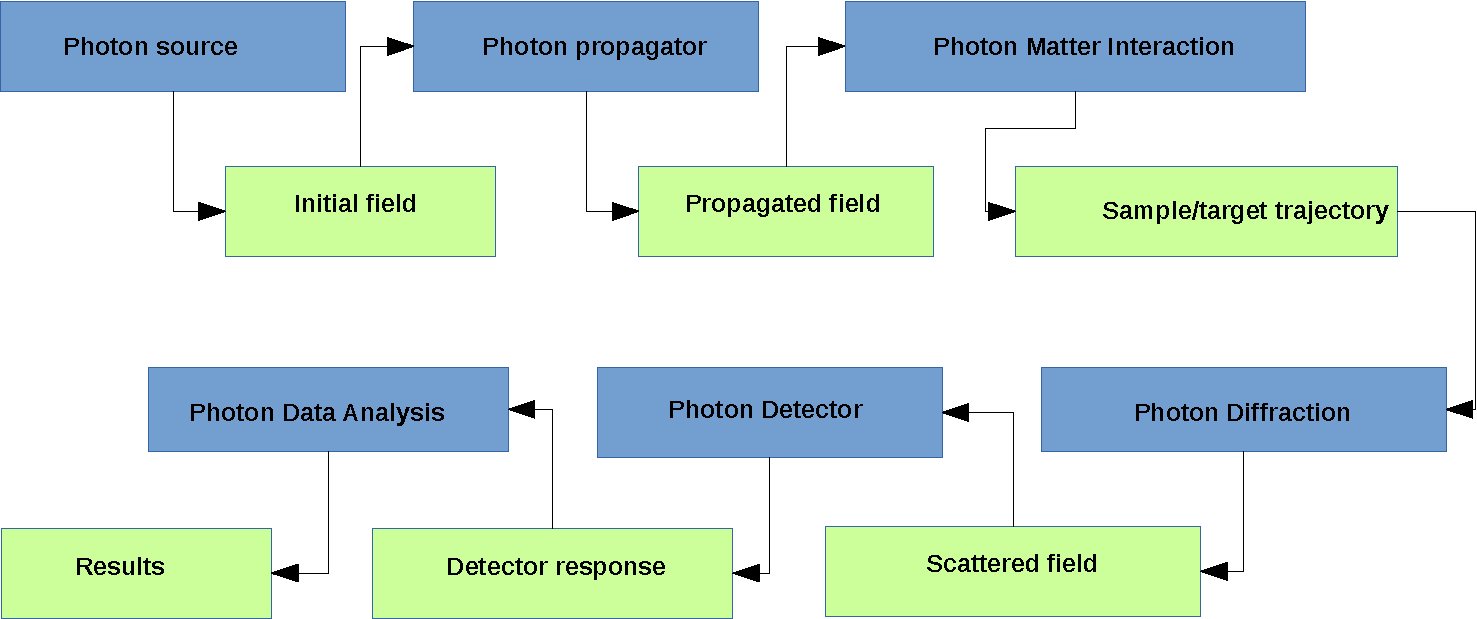
\includegraphics[width=1.0\textwidth,angle=0,clip]{simex_baseline_workflow-crop}
  \end{center}
\caption{Baseline workflow in \texttt{simex\_platform}. Blue boxes represent
\textit{Calculators}, green boxes are data interfaces.}
  \label{fig:simex_baseline_workflow}
\end{figure}

In it's current state, \texttt{simex\_platform} supports simulation of
photon experiments, that follow a linear base pattern: The radiation is produced
in a photon source, propagated through a beamline, it interacts with a sample
(target), and photons leaving the sample after scattering or emission are
detected in a photon detector. This linear progression, depicted in
Fig.~\ref{fig:simex_baseline_workflow} will be referred to as
the simulation  baseline in the following. A typical example is a x-ray diffraction
experiment: X-ray photons delivered by a synchrotron or an FEL, scatter from a
sample (e.g. a crystal), and the scattered or diffracted photons are captured in
an area detector behind the sample. Other baseline applications are e.g. small
and wide angle scattering, inelastic x-ray scattering, or x-ray absorption
spectroscopy. Simulation of experiments that are not directly
representable in this ordered linear pattern are possible but not supported in the same way and
to the same extent as baseline applications. E.g.
experiments that involve more than one photon source, or applications where
products from photon-matter interaction (e.g. accelerated electrons or ions) are
utilized for further interactions, such as laser-plasma based x-ray sources or
proton radiography using laser accelerated protons.

A baseline application encapsulates six parts:
The photon source, the photon transport from the source to the
experiment, the interaction of photons and matter, propagation of scattered and
transmitted radiation from the target/sample to the detector, photon
detection, an data analysis. In \texttt{simex\_platform}
each of these blocks is represented by a suitable \textit{Calculator}. A
\textit{Calculator} can be seen as an operator acting on the data representing
radiation. It reads data from an input, performs a calculation with the data,
potentially modifies the data based on the calculation results, and  writes the
modified or propagated radiation to its output. Calculators are organized in a
lightweight abstraction scheme, represented in Fig.~\ref{fig:simex_calculators_tree}.
\begin{figure}[ht]
  \begin{center}
    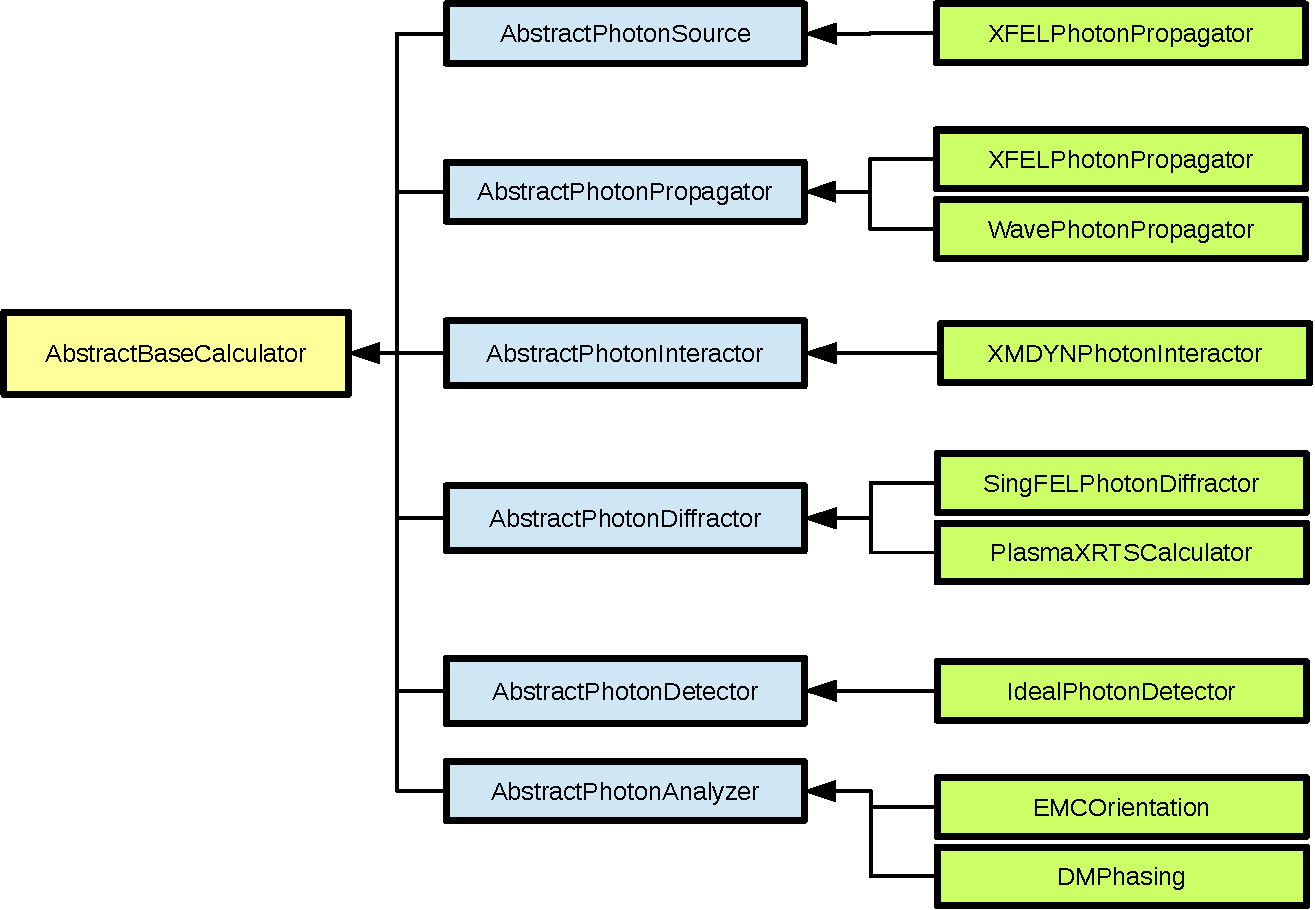
\includegraphics[width=1.0\textwidth,angle=0,clip]{calculators_inheritance-crop}
  \end{center}
  \caption{Inheritance tree for \textit{Calculators} in \texttt{simex\_platform}.}
  \label{fig:simex_calculators_tree}
\end{figure}

Commonalities between calculators are implemented on higher levels of
abstraction (blue or yellow boxes) whereas
specialities of each individual \textit{Calculator} are encapsulated in the
derived classes (green boxes). By providing as much functionality as possible on
the abstract level, the task of adding a new calculator to the set of existing
calculators is facilitated to a large degree, making \texttt{simex\_platform}
user friendly and opening collaborative opportunities also beyond EUCALL.


\subsection{Interfaces}
Start-to-end simulations in \texttt{simex\_platform} require that any two
subsequent \textit{Calculators} employed in the simulation pipeline can
communicate data amongst each other. The data source has to write the data in a
format that the data sink can handle and interpret correctly. In
\texttt{simex\_platform}, we chose the hdf5 \cite{hdf5} hierarchical data format
as the underlying format for all simulation data files. Data consistency in the
workflow is realized by each \textit{Calculator} defining the names of hdf
datasets and attributes that it requires to perform its calculation task and the
names of all datasets and attributes that it provides to the subsequent
calculator. In this way, after instantiating the \textit{Calculators} for a
simulation, the user or a workflow manager can check if the data can be
channeled through the \textit{Calculators} and give a feedback if there is a
mismatch between provided and expected data for two subsequent
\textit{Calculators}.


\subsection{Backengines}
The \textit{Calculators} in \texttt{simex\_platform} are mere user interfaces to
software executables or scripts that perform the actual mathematical operations on the
\textit{Calculator's} input data. In the following, we refer to these
executables and scripts as the \textit{Backengines}. One \textit{Calculator}
always wraps exactly one \textit{Backengine}, but one \textit{Backengine} can be
wrapped by more than one \textit{Calculator}.

\section{Documentation of \textit{Calculators} and their Interfaces}

An intermediate goal in SIMEX is to enable simulation of three distinct baseline
experiments:
\begin{enumerate}
  \item Single-particle imaging at the European XFEL (SPB-SFX instrument)
  \item Small-angle x-ray scattering from high power laser excited overdense
    plasmas (XFEL, HED instrument)
  \item Dynamic compression of solid matter using high energy lasers and x-ray
    absorption (ESRF, beamline ID24)
\end{enumerate}
We will now list the simulation codes (backengines), the interfaces and
\textit{Calculators} that have been developed to simulate these experiments.

\subsection{Photon source}
Description of the x-ray source.
\subsubsection{European XFEL}
\begin{description}
  \item[Backengine:] The code FAST \cite{Saldin1999} generates 3D (x-y-t) wavefronts at the exit of the undulator in an x-ray free electron laser.
  \item[Method:] 3D time resolved explicit solver for SASE FEL radiation
  \item[Provided data:]
\end{description}

\subsubsection{ESRF}
\begin{description}
  \item[Backengine:]
  \item[Method:]
  \item[Provided data:]
\end{description}

\subsection{Photon Propagation (Task 4.1.1)}
Propagates the radiation as described by the photon source calculator from the
source to the point of interaction with the sample or target under
investigation. Describes focussing, filtering, pulse shaping, and other optical
effects realized through lenses, mirrors, apertures, grids etc.
\subsubsection{European XFEL}
\begin{description}
  \item[Backengine:] WPG \cite{Samoylova2016, wpg_github}
  \item[Required data:]
  \item[Provided data:]
\end{description}
%
\subsubsection{ESRF}
\begin{description}
  \item[Backengine:] Shadow / Oasys
  \item[Required data:]
  \item[Provided data:]
\end{description}


\subsection{Photon Interactor (Task 4.1.2)}
Interaction of the photons with the target or sample. Takes into account
elementary processes like absorption, emission, scattering of radiation and
secondary processes like collisional ionization and recombination. The end
product is the electronic state of the sample/target as a function of time
during the interaction with the external light source.
\subsubsection{Single-particle imaging}
\begin{description}
  \item[Backengine:] XMDYN and XATOM: Molecular Dynamics and ab-initio
    electronic structure in intense x-ray fields \cite{Jurek2016, Son2013,
    Ziaja2015}
  \item[Required data:]
  \item[Provided data:]
\end{description}

\subsubsection{High-power laser\label{sec:hpl}}
\begin{description}
  \item[Backengine:] Particle in cell code PIConGPU \cite{Bussmann2013}
  \item[Required data:] Initial atom positions and optical laser parameters
    (pulse duration, focal spotsize, wavelength, pulse energy)
  \item[Provided data:] Electron density, atom positions, electromagnetic field
    as function in 6D phase space and time.
\end{description}
%
\subsubsection{High-energy laser}
\begin{description}
  \item[Backengine:] 1-D radiation hydrodynamic simulations
  \item[Required data:] Target specification (mass density profile, zone
    boundaries, initial temperature and pressure and optical laser parameters
    (pulse duration, focal spotsize, wavelength, pulse energy)
  \item[Provided data:] Mass density distribution, temperature, pressure and
    shock front velocity in 1D space as function of time.
    as function in 6D phase space and time.
\end{description}

\subsection{Photon Scattering and Diffraction (Task 4.1.3)}

\subsubsection{X-ray absorption fine structure}
\begin{description}
  \item[Backengine:] FEFF
  \item[Required data:] Rad-hydro output, ion structure (??)
  \item[Provided data:] Synthetic XAFS signal (??)
\end{description}

\subsubsection{X-ray radiography}
\begin{description}
  \item[Backengine:] Shadow \cite{}
  \item[Required data:] Rad-hydro output
  \item[Provided data:] Synthetic radiograph
\end{description}
\subsubsection{Ex-situ scattering}
\begin{description}
  \item[Backengine:] paraTaxis \cite{paraTaxis_github}
  \item[Required data:] PIC data (see \ref{sec:hpl}) and x-ray photon distribution
  \item[Provided data:] Synthetic diffraction image (photon count per pixel)
\end{description}

\subsubsection{Single-particle diffraction}
\begin{description}
  \item[Backengine:] SingFEL, implements 2nd order Born approximation scattering using via electronic form factors.
  \item[Required data:]
  \item[Provided data:]
\end{description}
%
\subsubsection{Plasma X-ray Thomson Scattering}
\begin{description}
  \item[Backengine:] XRTS, differential inelastic scattering cross section for scattering from warm and hot dense plasmas in various
    approximations \cite{Gregori2009, Fortmann2009d, Fortmann2010a}
  \item[Required data:]
  \item[Provided data:]
\end{description}
%
\subsection{Photon Detector (Task 4.1.4)}
\subsubsection{Pixel area detectors}
\begin{description}
  \item[Backengine:] X-ray camera simulation toolkit X-CSIT \cite{Joy2015}.
  \item[Required data:] Intensity or photon distribution at the detector.
  \item[Provided data:] Detector response to the signal, e.g. photons per pixel in an area detector.
\end{description}
%%
%\subsection{Photon Analysis}
%Following the detector readout, the recorded raw data has to be analyzed in
%order to extract the desired information about the target/sample. The specific
%algorithms depend largely on the details of the experiment and the underlying
%questions. Here, we discuss the analysis steps to be taken in a single particle
%diffractive imaging experiment.
%\begin{description}
  %\item[Abstract calculator:] AbstractPhotonAnalyzer
  %\item[Physics:]  Analysis of raw detector data. In SPI, the electron density
    %of the sample is reconstructed by assembling a 3D diffraction volume
    %from measured 2D diffraction patterns and subsequent phasing of the data to
    %solve the inverse scattering problem.
  %\item[Input data:] Detector response (raw data)
  %\item[Output data:] Reduced data to describe the investigated processes in the target/sample.
  %\item[Backengine:] Expand-Maximize-Compress (EMC)  for orientation,
    %Difference-Map for phasing \cite{Loh2009, s2e_recon_bitbucket}.
%\end{description}

\printbibliography
\end{document}


